\chapter{Additional Hardware Functions}

In addition to communication buses, described in chapter \ref{ch:hw_buses}, GEX implements several measurement and output functions that take advantage of the microcontroller's peripheral blocks, such as timers/counters and DAC. The more complicated ones are described here; simpler functions, such as the raw GPIO access, will be described later together with their control API.

\section{Frequency Measurement}

Applications like motor speed measurement and the reading of a VCO (voltage-controlled-oscillator) or VCO-based sensor's output demand a tool capable of measuring frequency. This can be done using a laboratory instrument such as the Agilent 53131A. A low cost solution is to use a timer/counter peripheral of a microcontroller, such as the STM32F072 used in GEX.

\begin{figure}
	\centering
	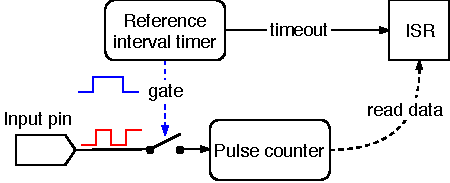
\includegraphics[scale=1] {img/fcap-direct.pdf}
	\caption{\label{fig:fcap-direct-dia}Direct frequency measurement method}
\end{figure}

\begin{figure}
	\centering
	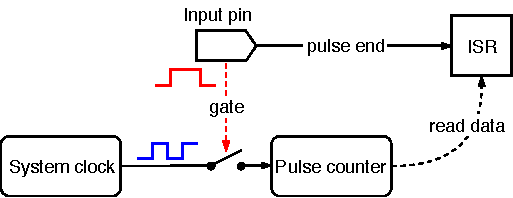
\includegraphics[scale=1] {img/fcap-reciprocal.pdf}
	\caption{\label{fig:fcap-reci-dia}Reciprocal frequency measurement method}
\end{figure}

\begin{figure}
	\centering
	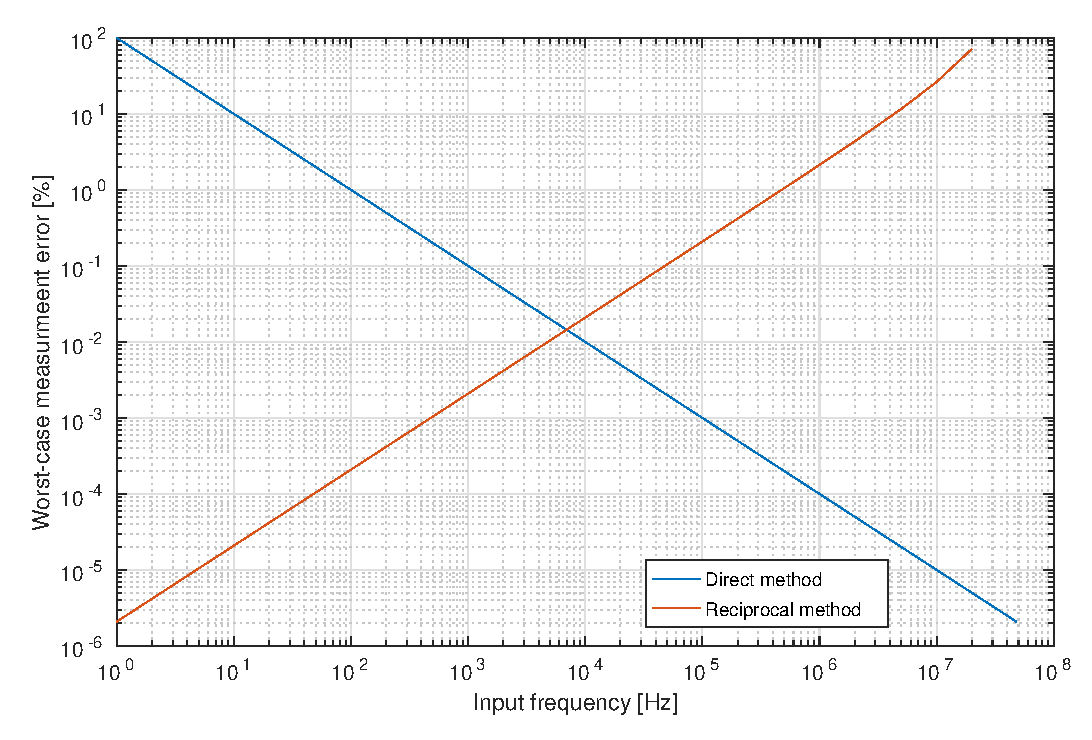
\includegraphics[width=.9\textwidth] {img/freqmethods.eps}
	\caption[Frequency measurement methods comparison]{\label{fig:freqmethods-graph}Worst-case error using the two frequency measurement methods with an ideal 48\,MHz timer clock. The crossing lies at 7\,kHz with an error of 0.015\,\%, or 1.05\,Hz.}
\end{figure}

Two basic methods to measure frequency exist, each with it's advantages and drawbacks:

\begin{itemize}
	\item The \textit{direct method} (fig. \ref{fig:fcap-direct-dia}) is based on the definition of frequency as a number of cycles $n$ in a fixed-length time window $\tau$ (usually 1\,s); the frequency is then calculated as $f=n/\tau$. 
	
	One timer generates the time window and its output gates the input of another, configured as a pulse counter. At the end of the measurement window an interrupt is generated and we can read the pulse count from the counter's register. 
	
	The direct method has a resolution of 1\,Hz with a sampling window of 1\,s (only a whole number of pulses can me counted). The resolution can be increased by using a longer time window, provided the measured signal is stable enough to make averaging possible without distorting the result.
	
	\item The \textit{indirect} or \textit{reciprocal method} (fig. \ref{fig:fcap-reci-dia}) measures one period $T$ as the time interval between two pulses and this is then converted to frequency as $f=1/T$. 
	
	This method needs only one timer/counter. Cycles of the system clock are counted for the duration of one period on the input pin (between two rising edges). If we additionally detect the falling edge in between, the counter's value gives us the duty cycle when related to the overall period length.
	
	Te reciprocal method's resolution depends on the counter's clock speed; if driven at 48\,MHz, the tick period is 20.83\,ns, which defines the granularity of our time measurement. It is common to measure several pulses and average the obtained values to further increase the precision. 
	
	We can easily achieve a sub-hertz resolution with this method, but its performance degrades at high frequencies where the time measurement precision becomes insufficient. The input frequency range can be extended using a hardware prescaller\footnote{\textit{Prescaller} is a divider implemented as part of the timer/counter peripheral block that can be optionally enabled and configured to a desired division factor.}, which is also applicable to the direct method, should the measurement of frequencies outside the counter's supported range be required. A duty cycle measurement available in this method can be used to read the output of sensors that use a pulse-width modulation.
\end{itemize}

Which method to use depends on the frequency we want to measure; the worst-case measurement errors of both methods, assuming an ideal 48\,MHz system clock, are plotted in figure \ref{fig:freqmethods-graph}. It can be seen that the reciprocal method leads in performance up to 7\,kHz where the direct method overtakes it. If a higher error is acceptable, the reciprocal method could be used also for higher frequencies to avoid a reconfiguration and to take advantage of its higher speed.

A good approach to a universal measurement, when we don't know the expected frequency beforehand, could be to first obtain an estimate using the direct method, and if the frequency is below the worst-case error crossing point (here 7\,kHz), to take a more precise measurement using the reciprocal method.

The system clock's frequency, which we use to measure pulse lengths and to gate the pulse counter, will be affected by tolerances of the used components, the layout of the PCB, temperature effects etc., causing measurement errors. A higher accuracy could be achieved using a temperature-compensated oscillator (TCO), or, in the direct method, by using the synchronization pulse provided by a GPS receiver to time the measurement interval.

\section{Waveform Generation with Direct Digital Synthesis}

\todo[inline]{todo}

